\section{Experiment}
\label{sec:experiments}

\subsection{Experimental Setup}

\paragraph{Implementation Details.}

We use Qwen2.5-VL 3B~\cite{bai2025qwen2} as the VLM backbone. The SFT stage runs for 1 epoch with batch size 64 and learning rate $1\text{e}{-5}$, followed by CoT-SFT for 15K iterations with the same hyperparameters. For teacher-student training, both $\mathcal{F}_\theta^T$ and $\mathcal{F}_\theta$ are initialized from the CoT-SFT checkpoint and trained for 4,500 iterations with batch size 128 and learning rate $1\text{e}{-6}$. The teacher is optimized with GRPO~\cite{shao2024deepseekmath} using action-aligned visual rewards~\cite{huang2025thinkact} and QA-style rewards (detailed in supplementary material). For the first 3,000 iterations of the student training, we train the verbalizer $\mathcal{V}_\psi$ with standard language modeling loss, then switch to $\mathcal{L}_{\text{verb}}$ for the remaining 1,500 iterations. For reasoning-enhanced policy learning, we initialize $\pi_\phi$ from DiT-Policy~\cite{chi2023diffusion} pre-trained on OXE~\cite{o2024open} for SimplerEnv, and from RDT~\cite{liu2024rdt} for LIBERO and RoboTwin2.0. A linear projection adapts the VLM's KV cache to the action model dimension (1,024 for DiT-Policy and 2,048 for RDT). Training runs for 20K iterations with batch size 256 and learning rate $1\text{e}{-4}$. All diffusion hyperparameters follow those of the respective action models. All experiments are conducted on 16 NVIDIA A100 GPUs with 80 GB memory.


\paragraph{Training Datasets and Evaluation Benchmarks.}

For reasoning VLM training, we utilize single-arm visual trajectories labeled by~\cite{lee2025molmoact} and dual-arm visual trajectories from the AIST dataset~\cite{aist2025aist}, along with QA tasks from PixMo~\cite{deitke2024molmo}, RoboFAC~\cite{lu2025robofac}, RoboVQA~\cite{sermanet2024robovqa}, ShareRobot~\cite{ji2025robobrain}, EgoPlan~\cite{chen2023egoplan}, and Video-R1~\cite{feng2025video}. For reasoning-enhanced policy learning, we use action data from the OXE dataset~\cite{o2024open} (following OpenVLA~\cite{kim24openvla}) when training with DiT-Policy, and augment with bimanual data from the static Aloha dataset~\cite{shi2023waypoint, zhao2023learning} when training with RDT.

We evaluate \ours{} on four embodied reasoning benchmarks and three robot manipulation benchmarks. For embodied reasoning, we use EgoPlan-Bench2~\cite{qiu2024egoplan2} (accuracy on multiple-choice questions), RoboVQA~\cite{sermanet2024robovqa} (BLEU score~\cite{papineni2002bleu}), OpenEQA~\cite{majumdar2024openeqa}, and RoboFAC~\cite{lu2025robofac} (both using LLM-based scoring). Notably, RoboVQA and RoboFAC contain videos captured from real robots. For robot manipulation, we evaluate on SimplerEnv~\cite{li24simpler}, which demonstrates strong correlation with real-world performance, LIBERO~\cite{liu2023libero} covering diverse manipulation tasks including long-horizon scenarios, and RoboTwin2.0~\cite{chen2025robotwin2} for complex bimanual manipulation. All robot manipulation tasks use task success rate as the metric. Additional details are provided in the supplementary material.

\subsection{Quantitative Evaluation}


\paragraph{Robot Manipulation.}

\begin{table*}[t!]
    \centering
    \caption{\textbf{Quantitative evaluation on RoboTwin2.0~\cite{chen2025robotwin2}.} E and H denote easy and hard settings (without/with domain randomization). Background colors indicate task length based on expert demonstrations: \colorbox{green!20}{short (80-100)}, \colorbox{yellow!20}{medium (110-220)}, \colorbox{red!20}{long (270-470)} steps.}
    \resizebox{\textwidth}{!}{%
        \begin{tabular}{l|
        cc|cc|cc|
        cc|cc|cc|
        cc|cc|cc|cc|cccc}
            \toprule
            \multirow{2}{*}{Model} 
            & \multicolumn{2}{c|}{\cellcolor{green!20}\makecell{click\\alarm}} 
            & \multicolumn{2}{c|}{\cellcolor{green!20}\makecell{click\\bell}} 
            & \multicolumn{2}{c|}{\cellcolor{green!20}\makecell{turn\\switch}} 
            & \multicolumn{2}{c|}{\cellcolor{yellow!20}\makecell{adjust\\bottle}} 
            & \multicolumn{2}{c|}{\cellcolor{yellow!20}\makecell{beat\\block}} 
            & \multicolumn{2}{c|}{\cellcolor{yellow!20}\makecell{handover\\mic}} 
            & \multicolumn{2}{c|}{\cellcolor{red!20}\makecell{handover\\block}} 
            & \multicolumn{2}{c|}{\cellcolor{red!20}\makecell{hanging\\mug}} 
            & \multicolumn{2}{c|}{\cellcolor{red!20}\makecell{stack\\blocks~two}} 
            & \multicolumn{2}{c|}{\cellcolor{red!20}\makecell{stack\\bowls~three}} 
            & \multicolumn{2}{c}{Average} \\
            \cmidrule{2-23}
            & \cellcolor{green!20}E & \cellcolor{green!20}H 
            & \cellcolor{green!20}E & \cellcolor{green!20}H 
            & \cellcolor{green!20}E & \cellcolor{green!20}H 
            & \cellcolor{yellow!20}E & \cellcolor{yellow!20}H 
            & \cellcolor{yellow!20}E & \cellcolor{yellow!20}H 
            & \cellcolor{yellow!20}E & \cellcolor{yellow!20}H 
            & \cellcolor{red!20}E & \cellcolor{red!20}H 
            & \cellcolor{red!20}E & \cellcolor{red!20}H 
            & \cellcolor{red!20}E & \cellcolor{red!20}H 
            & \cellcolor{red!20}E & \cellcolor{red!20}H 
            & E & H \\
            \midrule
            DP~\cite{chi2023diffusion} & 61 & 5 & 54 & 0 & 36 & 1 & 97 & 0 & 42 & 0 & 53 & 0 & 10 & 0 & 8 & 0 & 7 & 0 & 63 & 0 & 43.1 & 0.6 \\
            ACT~\cite{zhao2023learning} & 32 & 4 & 58 & 3 & 5 & 2 & 97 & 23 & 56 & 3 & 85 & 0 & 42 & 0 & 7 & 0 & 25 & 0 & 48 & 0 & 45.5 & 3.5 \\
            $\pi_0$~\cite{black2024pi_0} & 63 & 11 & 44 & 3 & 27 & 23 & 90 & 56 & 43 & 21 & 98 & 13 & 45 & 8 & 11 & 3 & 42 & 1 & 66 & 24 & 52.9 & 16.3 \\
            RDT~\cite{liu2024rdt} & 61 & 12 & 80 & 9 & 35 & 15 & 81 & 75 & 77 & 37 & 90 & 31 & 45 & 14 & 23 & 16 & 21 & 2 & 51 & 17 & 56.4 & 22.8 \\
            ThinkAct~\cite{huang2025thinkact} & 64 & 13 & 84 & 11 & 40 & 19 & 94 & 70 & 79 & 33 & 92 & 40 & 56 & 15 & 31 & 18 & 30 & 5 & 54 & 23 & 62.4 & 24.7 \\
            \midrule
            \textbf{\ours{}} & 70 & 17 & 82 & 12 & 37 & 21 & 92 & 72 & 82 & 33 & 99 & 42 & 65 & 15 & 30 & 22 & 45 & 5 & 55 & 25 & \textbf{65.7} & \textbf{26.4} \\
            \bottomrule
        \end{tabular}%
    }
    \label{tab:robotwin}
\end{table*}
\begin{table*}[t]
\centering
\caption{\textbf{Quantitative evaluation on EgoPlan-Bench2~\cite{qiu2024egoplan2}, RoboVQA~\cite{sermanet2024robovqa}, and OpenEQA~\cite{majumdar2024openeqa} benchmarks for embodied reasoning.}}
\resizebox{1.0\textwidth}{!}{
\small
\begin{tabular}{lccccccccccccc}
\toprule
\textbf{Method} & \multicolumn{5}{c}{\textbf{EgoPlan-Bench2}} & \multicolumn{5}{c}{\textbf{RoboVQA}} & \textbf{OpenEQA} & \cellcolor{gray!15}\textbf{Overall} \\
\cmidrule(lr){2-6} \cmidrule(lr){7-11}
 & Daily. & Work. & Rec. & Hobbies & Avg. & B-1 & B-2 & B-3 & B-4 & B-Avg. & Score & \cellcolor{gray!15}Avg. \\
\midrule
GPT-4V~\cite{achiam2023gpt} & 36.7 & 27.7 & 33.9 & 32.5 & 32.6 & 32.2 & 26.5 & 24.7 & 23.9 & 26.8 & 49.6 & \cellcolor{gray!15}36.4 \\
Gemini-2.5-Flash~\cite{comanici2025gemini} & 44.2 & 42.3 & 43.2 & 39.1 & 42.4 & 39.1 & 31.6 & 22.9 & 22.1 & 28.9 & 45.3 & \cellcolor{gray!15}38.9 \\
\midrule
InternVL2.5-2B~\cite{chen2024expanding} & 30.9 & 27.8 & 28.6 & 33.1 & 30.1 & 36.6 & 33.7 & 31.0 & 29.4 & 32.7 & 47.1 & \cellcolor{gray!15}36.6 \\
InternVL3-2B~\cite{zhu2025internvl3} & 36.9 & 29.9 & 35.6 & 31.5 & 33.4 & 34.4 & 33.9 & 33.5 & 33.3 & 33.8 & 48.8 & \cellcolor{gray!15}38.7 \\
NVILA-2B~\cite{liu2024nvila} & 34.6 & 26.7 & 33.3 & 31.6 & 31.4 & 38.7 & 34.3 & 31.1 & 29.2 & 33.3 & 47.0 & \cellcolor{gray!15}37.2 \\
Qwen2.5-VL-3B~\cite{bai2025qwen2} & 29.0 & 27.0 & 30.2 & 28.9 & 28.5 & 42.5 & 36.3 & 28.7 & 31.8 & 34.8 & 43.4 & \cellcolor{gray!15}35.6 \\
Magma-8B~\cite{yang2025magma} & 32.1 & 25.7 & 34.4 & 29.3 & 29.8 & 38.6 & 31.5 & 28.1 & 26.7 & 31.2 & 49.1 & \cellcolor{gray!15}36.7 \\
RoboBrain2.0-3B~\cite{team2025robobrain2} & 45.3 & 37.6 & 45.9 & 39.7 & 41.8 & 54.4 & 47.7 & 43.1 & 41.0 & 46.5 & 50.1 & \cellcolor{gray!15}46.1 \\
ThinkAct-3B~\cite{huang2025thinkact} & 46.6 & 41.4 & 45.9 & 42.5 & 44.0 & 62.4 & 57.3 & 52.0 & 49.6 & 55.3 & 48.9 & \cellcolor{gray!15}49.4 \\
\midrule
\textbf{Fast-ThinkAct-3B} & \textbf{50.3} & \textbf{44.3} & \textbf{46.4} & \textbf{43.2} & \textbf{46.4} & \textbf{70.1} & \textbf{63.0} & \textbf{57.2} & \textbf{53.0} & \textbf{60.8} & \textbf{51.2} & \cellcolor{gray!15}\textbf{52.8} \\
\bottomrule
\end{tabular}
}
\label{tab:egoplan_robo_results}
\vspace{-2mm}
\end{table*}

We evaluate \ours{} on robotic manipulation using LIBERO~\cite{liu2023libero} and SimplerEnv~\cite{li24simpler} benchmarks. LIBERO covers diverse subtasks, including Spatial, Object, Goal, and Long, while SimplerEnv provides a simulated benchmark with strong real-world correlation, featuring variations in lighting, object appearance, and camera viewpoints. As shown in Fig.~\ref{fig:libero_simpler}(a)-(e), \ours{} consistently outperforms all baselines, achieving the highest success rates across all LIBERO subtasks and SimplerEnv-Google. This includes substantial improvements over foundation VLAs such as OpenVLA~\cite{kim24openvla}, and reasoning VLAs including CoT-VLA~\cite{zhao2025cot}, ThinkAct~\cite{huang2025thinkact}, and MolmoAct~\cite{lee2025molmoact}. Moreover, as shown in Fig.~\ref{fig:libero_simpler}(f), our compact latent reasoning achieves 89.3\% and 88.0\% latency reduction compared to ThinkAct-7B~\cite{huang2025thinkact} and MolmoAct-7B~\cite{lee2025molmoact} respectively, and $7\times$ faster inference than ThinkAct-3B, demonstrating substantial efficiency gains without sacrificing performance.

To further validate \ours{} on more complex scenarios, we evaluate on RoboTwin2.0~\cite{chen2025robotwin2}, a challenging bimanual manipulation benchmark requiring long-horizon planning. As shown in Tab.~\ref{tab:robotwin}, \ours{} significantly outperforms previous VLAs including DP~\cite{chi2023diffusion}, ACT~\cite{zhao2023learning}, $\pi_0$~\cite{black2024pi_0}, RDT~\cite{liu2024rdt}, and ThinkAct~\cite{huang2025thinkact} across both easy and hard settings. Compared to RDT, \ours{} achieves 9.3\% and 3.6\% higher success rates on easy and hard settings, respectively. Against the reasoning VLA ThinkAct, it improves success by 3.3\% and 1.7\% while maintaining substantially higher efficiency, as shown in Fig.~\ref{fig:libero_simpler}(f). These results demonstrate that our compact reasoning design enables both superior accuracy and computational efficiency on complex bimanual manipulation tasks.



\paragraph{Embodied Reasoning.}

In Tab.~\ref{tab:egoplan_robo_results}, we evaluate the reasoning capabilities of \ours{} in embodied scenarios across three benchmarks: EgoPlan-Bench2~\cite{qiu2024egoplan2}, RoboVQA~\cite{sermanet2024robovqa}, and OpenEQA~\cite{majumdar2024openeqa}. These benchmarks assess multi-step planning in egocentric everyday scenarios, long-horizon reasoning for robotic manipulation tasks, and zero-shot understanding of embodied scenes in diverse environments, respectively. We observed that, \ours{} surpasses all comparison methods, including two proprietary models (i.e., GPT-4V~\cite{achiam2023gpt} and Gemini-2.5-Flash~\cite{comanici2025gemini}), exceeding the runner-up by 2.4\% on EgoPlan-Bench2, 5.5 BLEU score on RoboVQA, and 1.1 points on OpenEQA. These results demonstrate that \ours{} effectively handles complex planning sequences and extended reasoning horizons while generalizing to novel environments, showcasing robust capabilities for scene comprehension and multi-step task execution in embodied AI applications.


\begin{figure*}[t!]
    \centering
    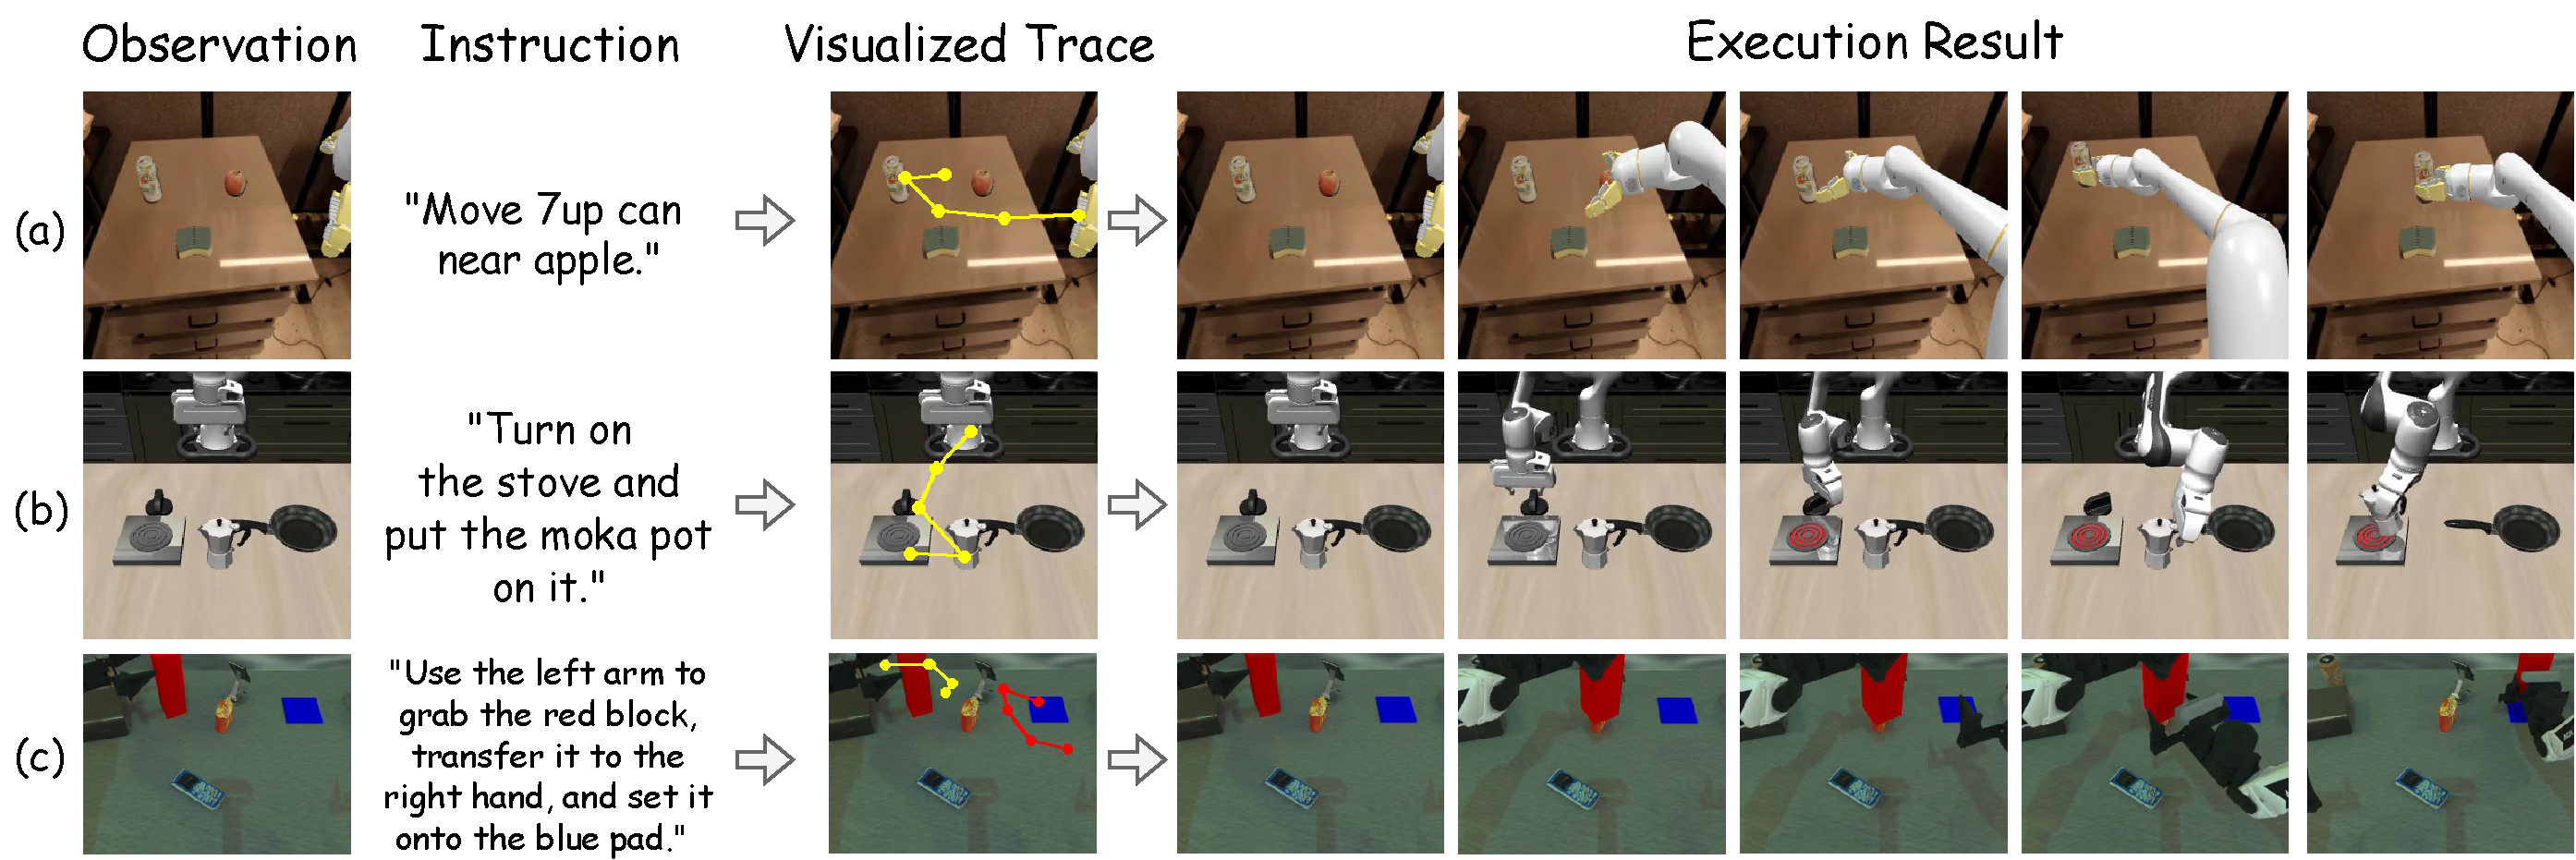
\includegraphics[width=1.0\linewidth]{figures/images/visualize_manipulation.pdf}
    \caption{\textbf{Visualization of predicted visual trajectories and action execution results on long-horizon tasks.} Examples from (a) SimplerEnv-Google, (b) LIBERO-Long, and (c) RoboTwin2.0-Hard with long (278) steps. Yellow traces indicate single-arm/left gripper trajectories; red traces indicate right gripper trajectories for bimanual tasks.}
    \vspace{-2mm}
    \label{fig:visualize_manipulation}
\end{figure*}

\begin{figure*}[t!]
    \centering
    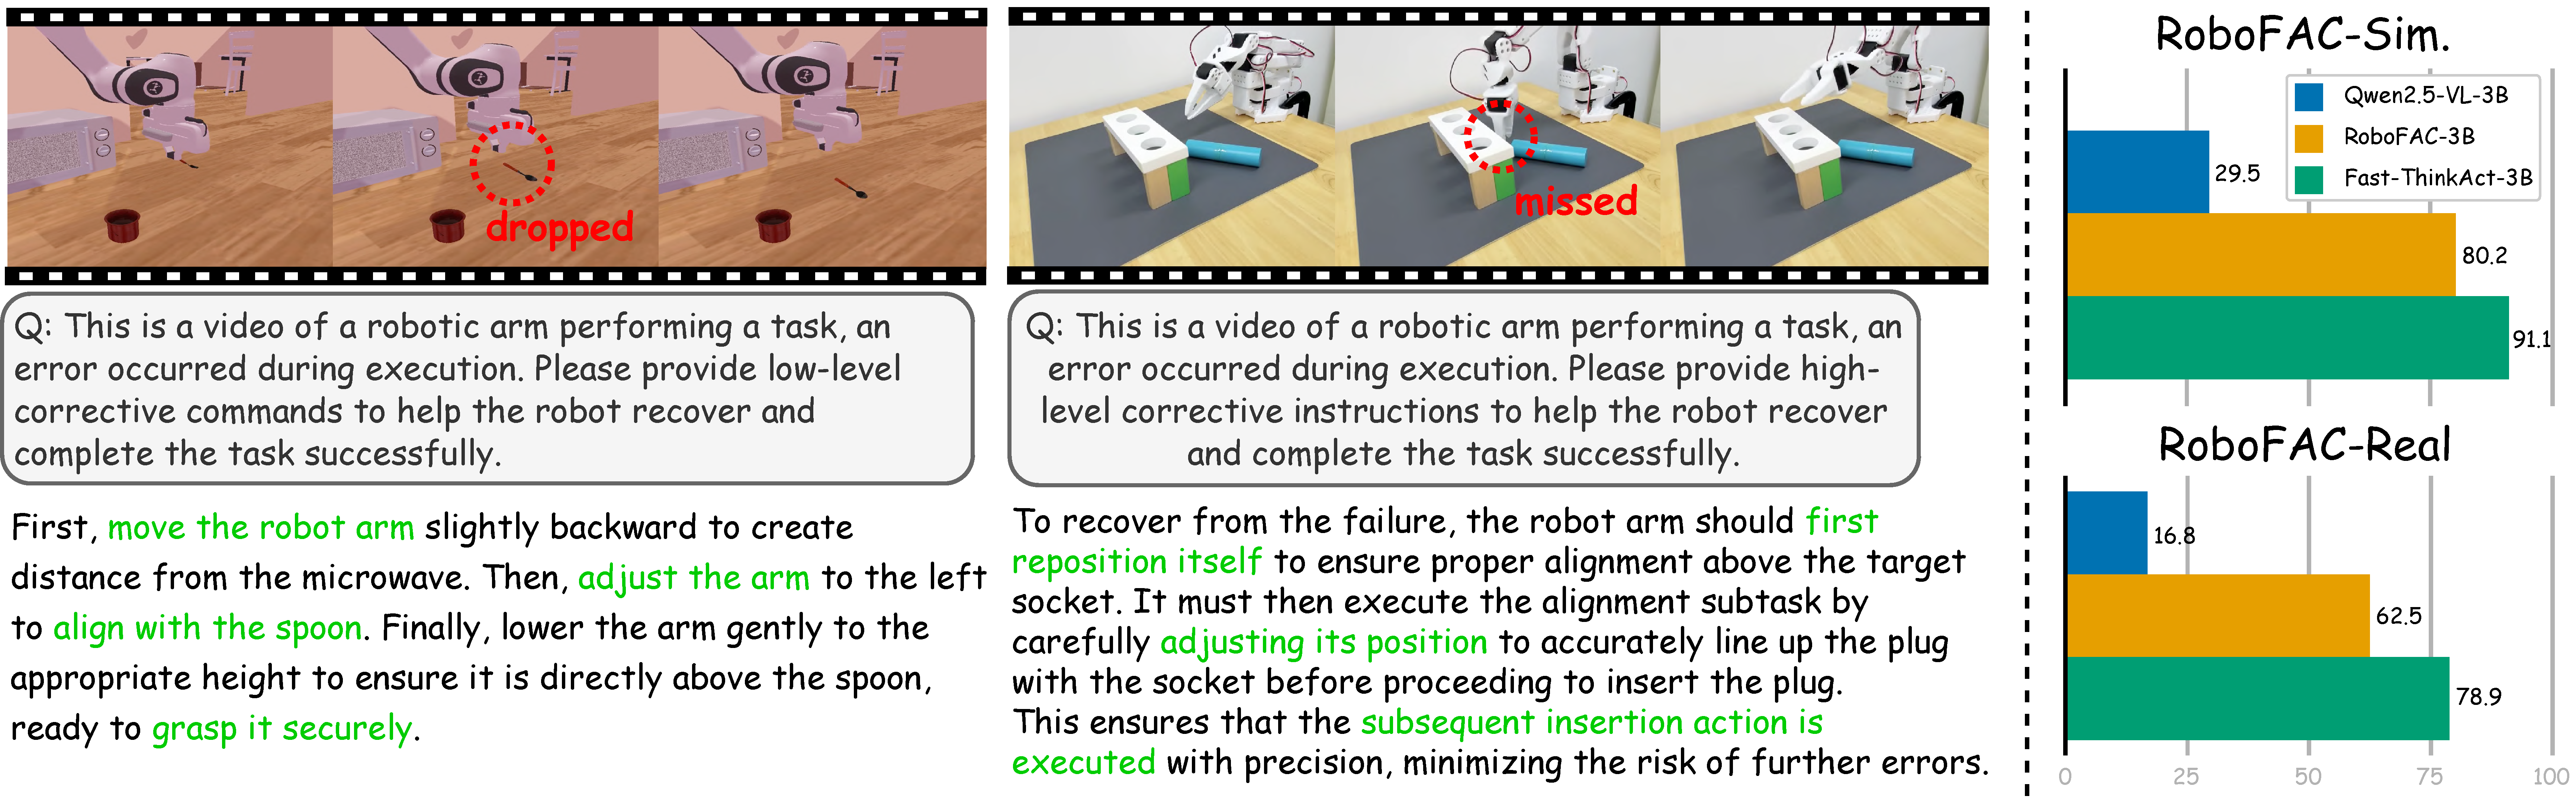
\includegraphics[width=1.0\linewidth]{figures/images/visualize_robofac.pdf}
    \vspace{-5mm}
    \caption{\textbf{Failure recovery capability on RoboFAC~\cite{lu2025robofac}.} Left: Qualitative examples (from both simulation and real robot) of corrective guidance for manipulation errors. Right: Quantitative evaluation on simulation (RoboFAC-Sim) and real-robot (RoboFAC-Real) settings.}
    \label{fig:visualize_robofac}
    % \vspace{-1mm}
\end{figure*}


\subsection{Analysis of Fast-ThinkAct}


\paragraph{Reasoning Enables Long-Horizon Planning.}

\begin{wrapfigure}{R}{0.45\textwidth}
    \centering
    \vspace{-3mm}
    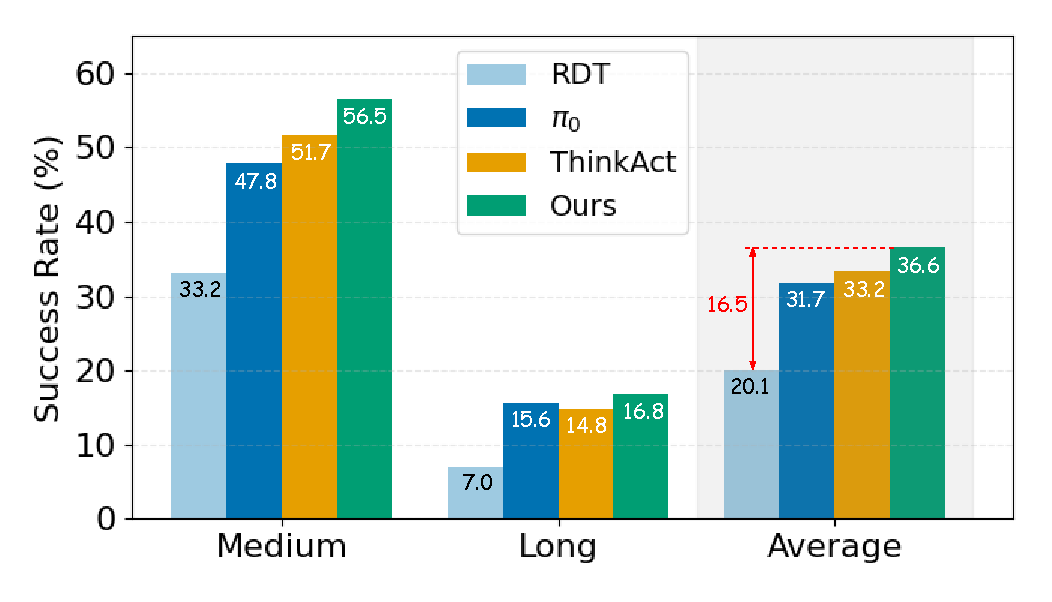
\includegraphics[width=\linewidth]{figures/images/exp_10shot.pdf}
    % \vspace{-3mm}
    \caption{\textbf{Few-shot adaptation results on RoboTwin2.0 benchmark.} We use 10 demonstrations per task for fine-tuning.}
    \label{fig:exp_10shot}
\end{wrapfigure}


We analyze \ours{}'s capability on long-horizon tasks in Tab.~\ref{tab:robotwin} and Fig.~\ref{fig:visualize_manipulation}. We focus on long-horizon tasks (average length exceeding 270 steps) in RoboTwin2.0~\cite{chen2025robotwin2} that require multi-step reasoning and extended planning horizons. As shown in Tab.~\ref{tab:robotwin}, \ours{} achieves average scores of 48.8 and 16.8 on easy and hard settings of long-horizon tasks, respectively, surpassing RDT (35.0/12.3) and ThinkAct (42.8/15.3). Fig.~\ref{fig:visualize_manipulation} visualizes predicted 2D visual traces and execution results on representative tasks from SimplerEnv-Google~\cite{li24simpler}, LIBERO-Long~\cite{liu2023libero}, and RoboTwin2.0~\cite{chen2025robotwin2}. For example, the LIBERO-Long task requires sequentially turning on the stove and placing a moka pot on it, while the RoboTwin2.0 handover task requires bimanual coordination to transfer a block between grippers. The visual traces successfully predict feasible solution paths, with their corresponding representations serving as visual planning guidance for successful execution. These results demonstrate that our compact latent reasoning effectively supports long-horizon planning in complex manipulation scenarios.

\paragraph{Reasoning Enables Failure Recovery.}

\begin{wrapfigure}{R}{0.5\textwidth}
    \centering
    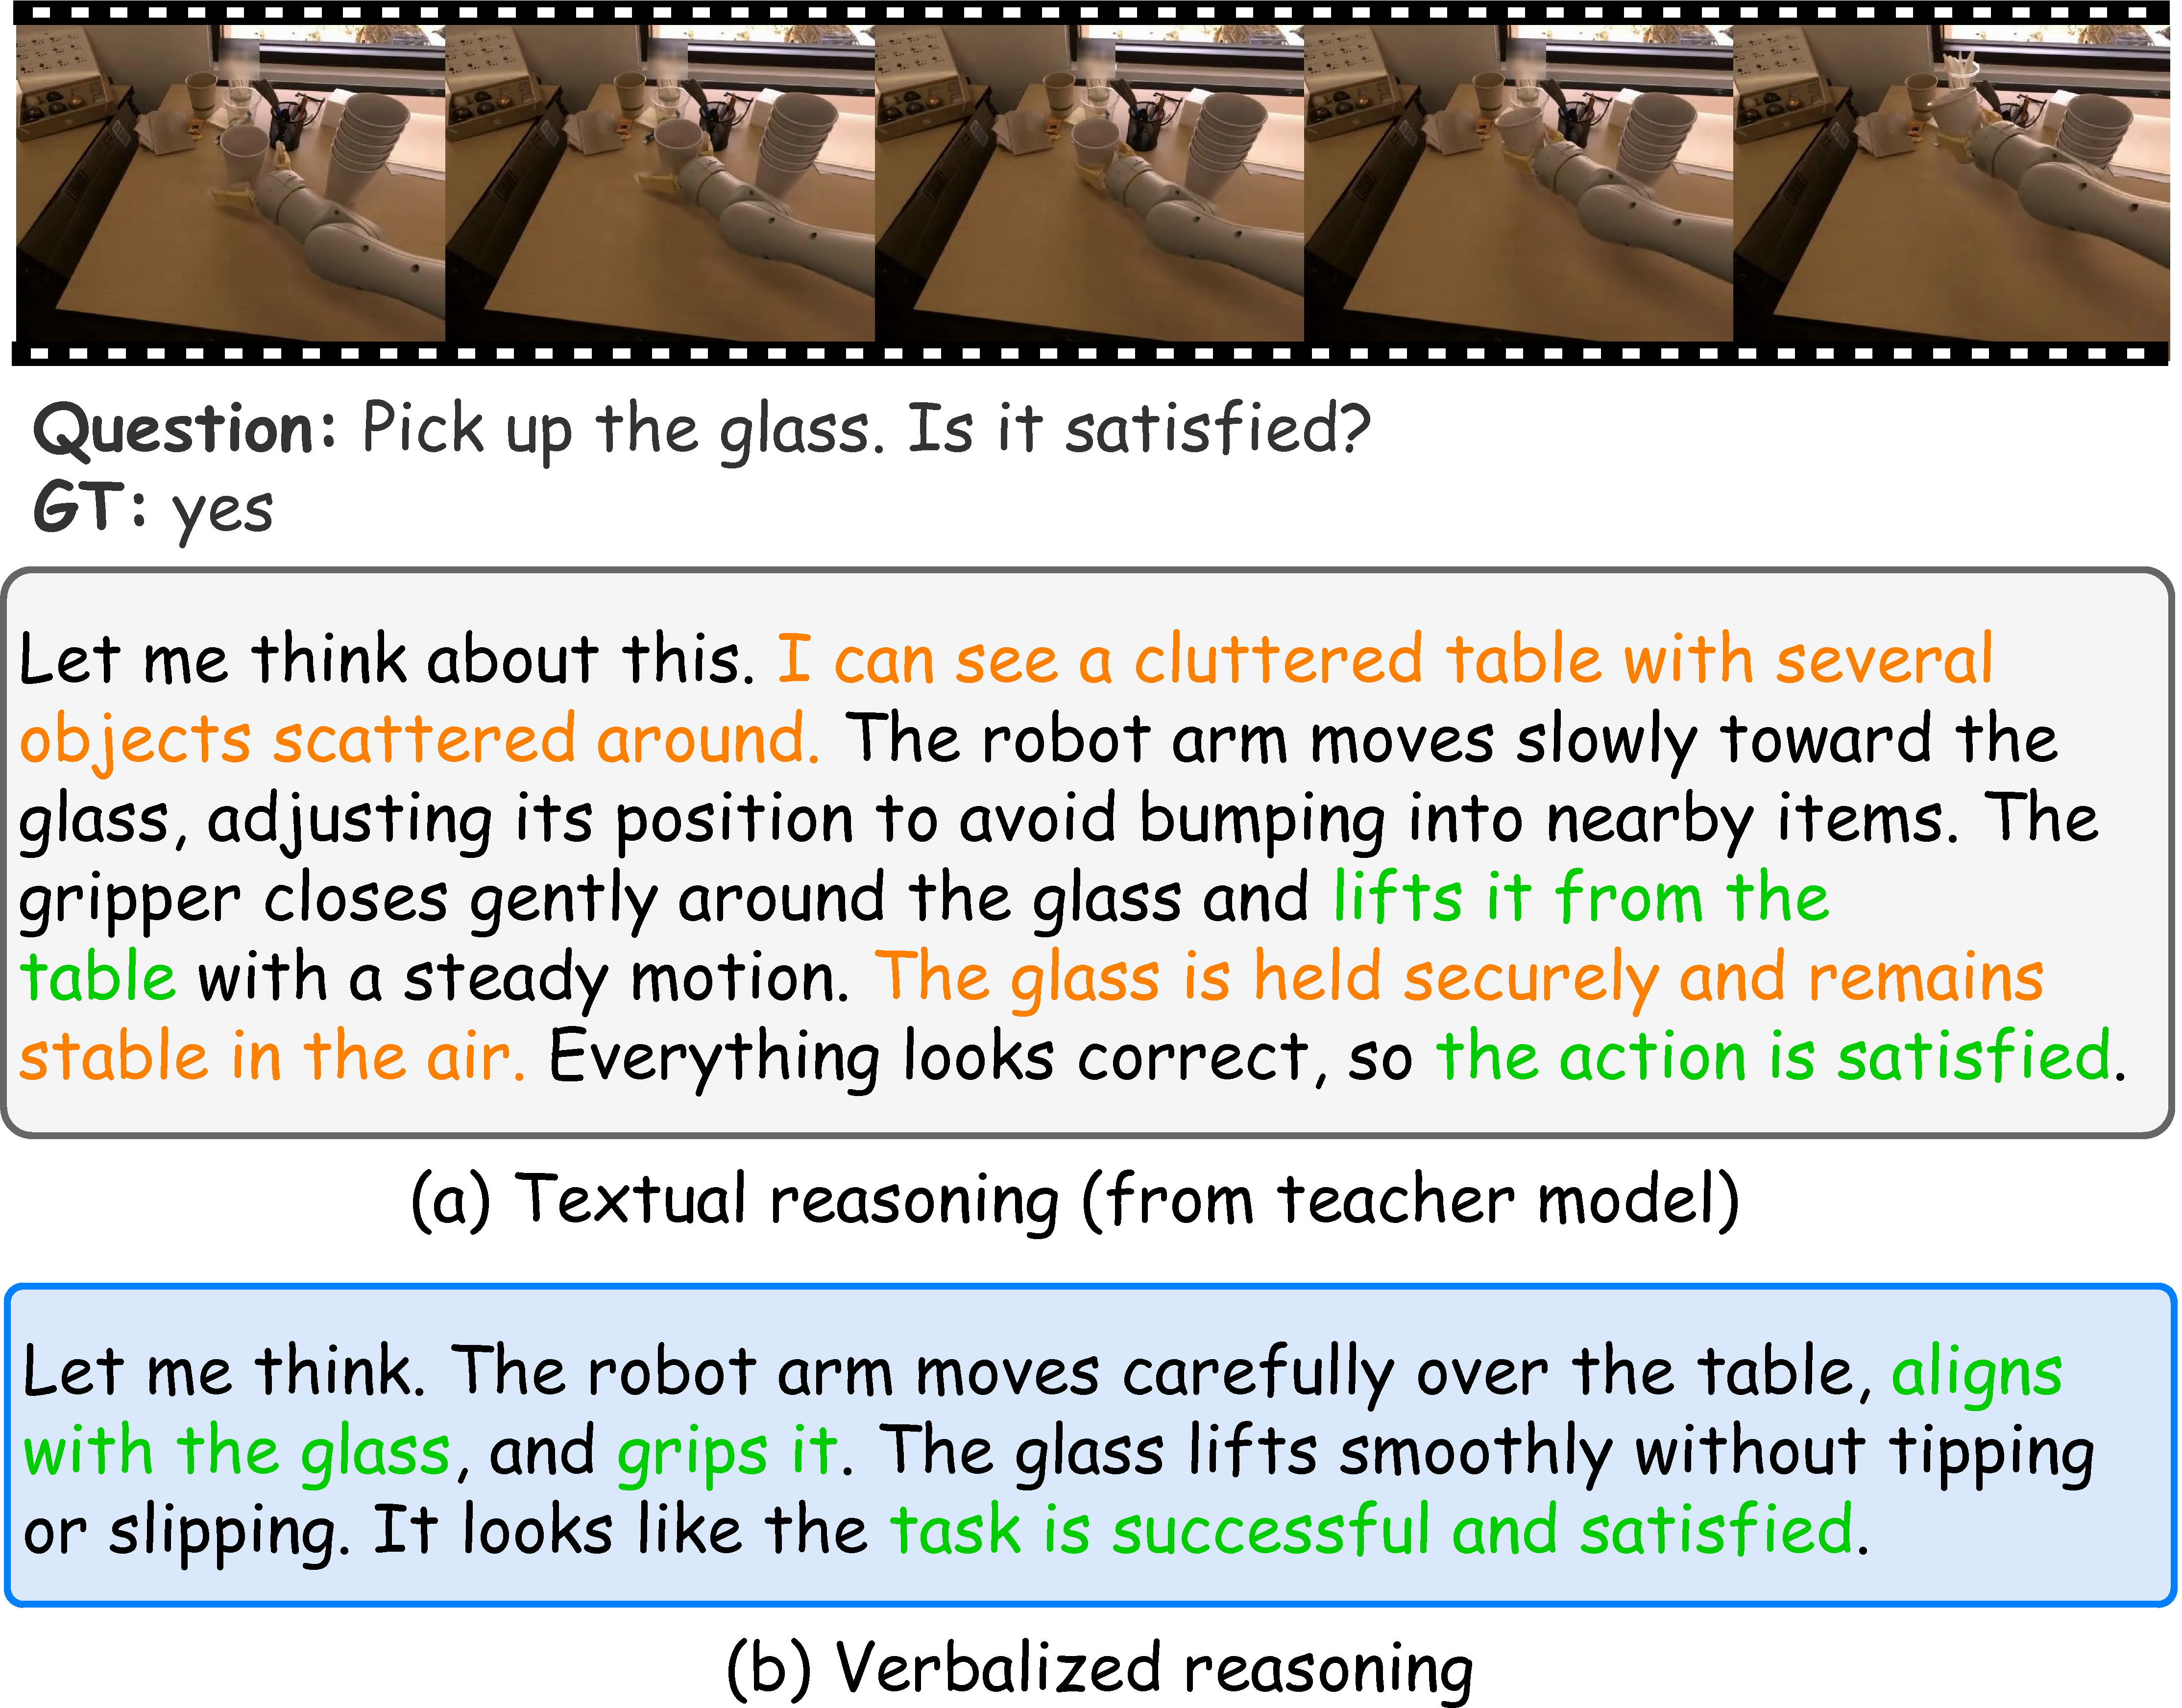
\includegraphics[width=1.0\linewidth]{figures/images/visualize_reasoning.pdf}
    \caption{\textbf{Reasoning trace comparison on RoboVQA.} (a) Teacher's textual reasoning. (b) Student's verbalized latent reasoning. \textcolor{YellowGreen}{Green}: relevant content; \textcolor{orange}{orange}: less relevant content.}
    \label{fig:visualize_reasoning}
    % \vspace{-15mm}
\end{wrapfigure}


A key advantage of reasoning-based VLAs~\cite{huang2025thinkact,abdolmaleki2025gemini} is their ability to identify runtime failures and provide corrective guidance for recovery. To evaluate this capability, we conduct experiments on RoboFAC~\cite{lu2025robofac}, a benchmark specifically designed to assess failure identification and correction in embodied VLMs. As shown in Fig.~\ref{fig:visualize_robofac}, \ours{} substantially outperforms the second-best baseline RoboFAC-3B~\cite{lu2025robofac} by 10.9 points on the simulation split and 16.4 points on the real-world split. The qualitative examples demonstrate \ours{}'s ability to reason over manipulation videos, identify failures, and propose recovery steps. For instance, in the right example where the target object drops mid-execution, \ours{} generates a concrete recovery plan: first moving the arm backward to create space, then adjusting laterally to align with the target object, and finally lowering to the appropriate height for a secure grasp. These results demonstrate that our latent reasoning supports both fast task execution and crucial failure analysis capabilities essential for robust robotic manipulation.

\paragraph{Reasoning Enables Few-Shot Adaptation.}

\begin{wraptable}{R}{0.55\textwidth}
    \centering
    \caption{\textbf{Ablation study of training objectives and learning stages.} Note that Fast-ThinkAct w/o $\mathcal{L}_{\text{verb}}, \mathcal{L}_{\text{distill}}$ denotes the student VLM $\mathcal{F}_\theta$ trained without the corresponding loss components.}
    \resizebox{\linewidth}{!}{
        \begin{tabular}{lcccc}
            \toprule
            \textbf{Method} & \textbf{EgoPlan} & \textbf{RoboVQA} & \textbf{OpenEQA} & \textbf{Average} \\
            \midrule
            \textbf{\ours{}} & \textbf{46.4} & \textbf{60.8} & \textbf{51.2} & \textbf{52.8} \\
            \midrule
            \; w/o $\mathcal{L}_\text{verb}$ & 42.1 & 53.8 & 49.5 & 48.5 \\
            \; w/o $\mathcal{L}_\text{verb},\mathcal{L}_\text{distill}$ & 41.6 & 52.7 & 48.9 & 47.7 \\
            \midrule
            Textual Teacher $\mathcal{F}_\theta^T$ & 41.7 & 58.2 & 49.4 & 49.8 \\
            SFT + CoT-SFT & 40.0 & 46.1 & 48.8 & 45.0 \\
            SFT only & 40.5 & 53.6 & 45.3 & 46.5 \\
            \bottomrule
        \end{tabular}
    }
    % \vspace{-0.5mm}
    \label{tab:ablation_stage_loss}
\end{wraptable}


To assess how reasoning capability improves few-shot adaptation, we conduct few-shot experiments on the RoboTwin2.0 benchmark~\cite{chen2025robotwin2}, fine-tuning models using only 10 demonstrations per task. As illustrated in Fig.~\ref{fig:exp_10shot}, \ours{} significantly enhances our adopted action model RDT~\cite{liu2024rdt} and outperforms the state-of-the-art VLAs, including $\pi_0$~\cite{black2024pi_0} and ThinkAct~\cite{huang2025thinkact} on both medium and long-horizon tasks. Notably, our method achieves these gains while operating with significantly lower reasoning latency compared to ThinkAct, highlighting the advantage of efficient yet effective reasoning for few-shot action adaptation in complex robot manipulation scenarios.

\paragraph{Visualization of Verbalizable Latent Reasoning.}
In Fig.~\ref{fig:visualize_reasoning}, we compare the teacher's textual reasoning with the student's verbalized latent reasoning on RoboVQA. While both capture task-relevant information (\textcolor{YellowGreen}{green}), the teacher generates verbose outputs with less directly relevant content (\textcolor{orange}{orange}), whereas our student produces more concise and focused responses when verbalized. This demonstrates that our preference-guided distillation not only reduces computational cost but also distills concise reasoning patterns while filtering out redundant information.


\paragraph{Ablation Study.}

In Tab.~\ref{tab:ablation_stage_loss}, we ablate training stages and loss components. Starting from the full \ours{}, removing $\mathcal{L}_\text{verb}$ causes performance drops as latent CoTs lack preference-based guidance to align with high-quality reasoning and suppress low-quality patterns. Further removing $\mathcal{L}_\text{distill}$ leads to additional decline, indicating that aligning trajectory-level representations is crucial for transferring visual planning capabilities. Comparing training strategies, CoT-SFT underperforms SFT on EgoPlan-Bench2 and RoboVQA but improves on OpenEQA, suggesting naïve chain-of-thought supervision benefits open-ended QA but introduces verbosity that hinders structured reasoning tasks. Our preference-guided approach distills high-quality reasoning while maintaining efficiency. This validates the necessity of our proposed distillation framework and visual trajectory alignment. We provide additional ablation studies in the supplementary material.

